\documentclass[preprint,12pt]{elsarticle}

\usepackage{amsmath}
\usepackage{amssymb}
\usepackage{graphicx}
\usepackage{booktabs}
\usepackage{tabularx}
\usepackage{array}
\usepackage{makecell}
\usepackage{multirow}
\usepackage{xcolor}
\usepackage{url}

\graphicspath{{figures/}}

% --------------------------------------------------------------
% DRAFT-ONLY ANNOTATIONS. Flip to \showtasksfalse for submission.
% --------------------------------------------------------------
\newif\ifshowtasks
\showtaskstrue

\newcommand{\TODO}[1]{\ifshowtasks\textcolor{red}{\textbf{[TODO: #1]}}\fi}

\journal{Artificial Intelligence in Medicine}

\begin{document}

\begin{frontmatter}

\title{Knowledge-Based Temporal Abstractions Transfer Across Hospitals:
A Seven-Arm Comparison of Complication Prediction on a Six-Hospital
Inpatient-Diabetes Cohort}

\author[aff1]{Shahar Oded\corref{cor1}}
\ead{shahar.oded@post.bgu.ac.il}
\cortext[cor1]{Corresponding author.}
\author[aff1]{Yuval Shahar}
\author[aff1]{Erez Shalom}
\author[aff2,aff3]{Amir Bashkin}
\author[aff4,aff5]{Leonard Saig}
\author[aff6]{Dror Cantrell}
\author[aff7]{Irit Wirsansky}
\author[aff2,aff8]{Muhamad Badarne}
\author[aff9]{Irena Barash}
\author[aff10,aff11]{Avivit Cahn}
\author[aff4,aff7]{Irit Hochberg}

\address[aff1]{Medical Informatics Research Center,
Ben-Gurion University of the Negev, Beer Sheva, Israel}
\address[aff2]{Azrieli Faculty of Medicine,
Bar-Ilan University, Safed, Israel}
\address[aff3]{Endocrinology and Diabetes Unit,
Galilee Medical Center, Nahariya, Israel}
\address[aff4]{Bruce Rappaport Faculty of Medicine,
Technion---Israel Institute of Technology, Haifa, Israel}
\address[aff5]{Endocrinology Institute,
Bnai Zion Medical Center, Haifa, Israel}
\address[aff6]{Internal Medicine Department C,
Shamir Medical Center, Beer Yaakov, Israel}
\address[aff7]{Endocrinology Unit,
Hillel Yaffe Medical Center, Hadera, Israel}
\address[aff8]{Endocrinology and Diabetes Service,
Tzafon Medical Center, Ramat Poriya, Israel}
\address[aff9]{Internal Medicine Department C,
Barzilai Medical Center, Ashkelon, Israel}
\address[aff10]{Internal Medicine Department A,
Hadassah Ein Kerem, Jerusalem, Israel}
\address[aff11]{Faculty of Medicine,
Hadassah Hebrew University Hospital, Jerusalem, Israel}

\begin{abstract}
\textbf{Background.} Interval-based Transformers over knowledge-based
temporal abstractions (KBTA) outperform strong neural baselines for
short-horizon complication prediction on a MIMIC-IV diabetic cohort, and
concurrent work has shown that adherence to inpatient hyperglycemia guideline
recommendations can be measured automatically as continuous compliance scores
over the same abstraction stream. Whether either result transfers to a
second, independently collected cohort, and whether the two signals combine
usefully, has not previously been examined.

\textbf{Objective.} To evaluate the transferability of INTERVenE-Enc across
health systems and knowledge bases, to test whether measured
guideline-adherence signals improve predictive performance beyond the
clinical record they were derived from, and to quantify the marginal
contribution of clinical domain knowledge to short-horizon complication
prediction on inpatient diabetes.

\textbf{Methods.} We conducted a retrospective comparison on the Kineret
inpatient hyperglycemia cohort ($48{,}354$ admissions across six Israeli
hospitals, August 2022--December 2025). A single seven-arm ladder holds
cohort, labels, patient split and evaluation window constant and varies only
the input representation: (i) logistic regression on distribution-summarized
raw measurements, (ii) ss-STraTS on the raw event stream, (iii) INTERVenE-Enc
on knowledge-free $\sigma$-bin intervals, (iv) INTERVenE-Enc on KBTA
intervals, and (v) the same with treatment-quality (QA) pattern tokens.
Every arm predicts three targets per complication: whether it occurs, when,
and length of stay. Confidence intervals are $2{,}000$-resample
patient-level bootstraps.

\textbf{Results.} On $4{,}686$ held-out test admissions, INTERVenE-Enc on KBTA
intervals achieves support-weighted AUPRC $0.527$ [$0.511, 0.548$] against
$0.472$ [$0.456, 0.493$] for the best raw-stream baseline (ss-STraTS), with
non-overlapping confidence intervals, and leads every arm on AUROC and onset
error. Replacing KBTA with $\sigma$-bins costs $0.073$ AUPRC and drops the
arm to the logistic-regression floor---a lift that was within noise on
MIMIC-IV. The QA block leaves aggregate metrics within third-decimal-place
noise on every model, though sparse-transcoder attribution shows that the
compliance-pattern tokens are among the top drivers for seven of eight
outcomes when INTERVenE receives them as intervals.

\textbf{Conclusion.} The architecture transfers, and the knowledge base does
predictive work on data it was authored for---not merely interpretive work
as on MIMIC-IV. Automatically measured guideline adherence carries little
information the interval stream does not already supply, because both are
deterministic derivations of the same abstraction layer. The design that
separates them---a seven-arm ladder with identical cohort, labels and
split---is what let the two effects be read against one another.
\end{abstract}

\begin{keyword}
temporal abstraction \sep clinical prediction \sep interval-based Transformer
\sep knowledge base \sep guideline adherence \sep transferability
\sep inpatient diabetes
\end{keyword}

\end{frontmatter}

\IfFileExists{tasks.tex}{% =====================================================================
% Draft-only task list. Rendered as a red box on the title page while
% \showtaskstrue; hidden by \showtasksfalse. Not part of the manuscript
% and excluded from the word count.
% =====================================================================
\label{sec:tasks-open}

\begin{center}
\fbox{\parbox{0.94\textwidth}{%
\textbf{\textcolor{red}{OPEN ITEMS BEFORE SUBMISSION}}\\[.4em]
\footnotesize

\textbf{A. Cross-references to companion papers}\\
Three placeholder bib keys are used throughout:
\texttt{oded2026intervene} (the AAAI methodological paper),
\texttt{oded2027kineret-jbi} (the JBI adherence paper), and
\texttt{mediator-github}. Update these to the accepted / preprint form
once the two companion drafts are placed. The \emph{Background} section
also references the JBI paper's Table~1 for cohort characteristics; if
JBI is not yet publicly citeable, reproduce the table as an appendix
here.\\[.2em]

\textbf{B. Empirical additions}\\
The following extensions are being staged in the Kineret-Prediction
repository. Items marked \emph{[inference-only]} reuse the existing
per-arm checkpoints and do not require retraining.
\begin{itemize}\setlength{\itemsep}{.05em}
  \item \emph{[inference-only]} Sensitivity of the ladder ordering to
        $K_{\mathrm{eval}} \in \{2, 3, 5, 6\}$. Because training augments
        over $K \in 1\ldots 13$, each trained checkpoint can be re-scored
        at any $K_{\mathrm{eval}}$ by cutting the same test admissions at
        a different point; no retraining is required.
  \item \emph{[inference-only]} Reliability curves and per-outcome ECE
        (with optional temperature scaling on validation), as reported
        for INTERVenE-Enc on MIMIC-IV in \citep{oded2026intervene}.
        Predictions live in \texttt{results/full\_bench\_results/runs/<arm>/}.
  \item \emph{[inference-only]} Age-band and sex subgroup AUROC/AUPRC
        (item C below); paired-bootstrap $\Delta$ and BH-FDR across
        outcomes (item D). Both from the existing predictions.
  \item \emph{[requires re-run]} Temporal held-out: retrain the ladder
        on pre-guideline admissions and evaluate on post-guideline (or
        vice versa), to test whether prediction quality tracks the
        practice shift documented in the JBI companion paper. Supported
        natively by the pipeline via \texttt{date\_range\_start} /
        \texttt{date\_range\_end}.
  \item \emph{[requires re-run]} Per-hospital leave-one-out for the KB
        arm (six re-runs), to quantify site generalization. Requires the
        hospital column to be plumbed through cohort assembly; check
        \texttt{Kineret-Prediction} PR before running.
  \item \emph{[inference-only]} Sparse-transcoder attribution
        reproduction on the KB+QA arm on this cohort. A partial run
        exists under \texttt{results/transformers-results-old-with-xai/}
        for pre-ladder ss-STraTS variants; the KB+QA reproduction reuses
        the pipeline documented in \citep{oded2026intervene}.
  \item \emph{Optional.} Multi-seed variance for the KB and KB+QA arms.
        The AAAI companion paper explicitly declined multi-seed at this
        cohort scale, on cost grounds, and reported patient-level
        bootstrap intervals only; we adopt the same stance and mention
        it as a limitation.
\end{itemize}
\vspace{.1em}

\textbf{C. Fairness / subgroup analyses}\\
AIIM reviewers routinely ask for at least age-band and sex subgroup
AUROC/AUPRC. The cohort is $54.3\%$ male and skewed older; a
per-subgroup table for the KB arm is one bootstrap run away.\\[.2em]

\textbf{D. Statistical practice}\\
\begin{itemize}\setlength{\itemsep}{.05em}
  \item Decide whether to report $P$ values for pairwise arm comparisons
        (currently only overlap-of-CIs is used). If so, the paired
        bootstrap $\Delta$ distribution is already computed for
        Figure~\ref{fig:qa-delta}; extend to all pairs.
  \item Multiple-testing correction across the eight per-outcome
        comparisons in Table~\ref{tab:per-outcome} (BH-FDR at $q<0.05$
        matches the JBI paper's convention).
\end{itemize}
\vspace{.1em}

\textbf{E. Author contributions and funding}\\
Funding statement outstanding (aligned with JBI/JAMIA companion
papers); ORCID identifiers to be added for all authors.\\[.2em]

\textbf{F. Figure budget}\\
AIIM allows up to $\sim 10$ figures without special permission. The
current draft uses $5$. Candidates for expansion: (i) event-reconciliation
diagram of the raw-vs-Mediator alignment pipeline (methods section);
(ii) sparse-transcoder attribution panel for the KB+QA arm;
(iii) per-outcome AUROC alongside AUPRC (data exists as
\texttt{fig4\_per\_target\_auroc.pdf} but is not included in the current
draft). Add if space permits after the empirical additions in item B.\\[.2em]

\textbf{G. Language and prose}\\
The draft borrows phrasing from the concurrent JBI/JAMIA drafts by
design (shared methods sections). Before submission, run a self-plagiarism
check against those two documents; substantive text overlap should
either be paraphrased or attributed as a shared methods description.
The abstract is currently unstructured. AIIM does not require a
structured abstract but common editorial policy is to prefer one; consider
converting to Objective / Methods / Results / Conclusion form.\\[.2em]

\textbf{H. Compilation}\\
Not yet built --- no TeX distribution here. Before submission, compile
end-to-end with \texttt{pdflatex} + \texttt{bibtex} and reconcile any
line-breaking / hyphenation issues in the tables. Confirm figure
placement floats do not push results captions past their referring
paragraph.
}}
\end{center}

\clearpage
}{}

\section{Introduction}
\label{sec:intro}

Short-horizon complication prediction from irregular electronic health record
(EHR) streams has been driven by two lines of work with an unresolved
intersection. On one side, sequence models---GRU-D
\citep{che2018recurrent}, STraTS \citep{tipirneni2022strats}, visit-level
Transformers such as BEHRT \citep{li2020behrt}, TransformEHR
\citep{yang2023transformehr}---operate on raw measurement streams and
extract clinically meaningful signal without explicit medical knowledge,
paying the cost that their attributions resolve to raw variables rather
than to clinical concepts. On the other, symbolic pipelines built on
knowledge-based temporal abstraction (KBTA) \citep{shahar1997framework}
convert raw observations into named clinical intervals---states, trends,
events, contexts---that support downstream mining (e.g., KarmaLego
\citep{moskovitch2015karmalego}) or scoring, at the cost of a curated
knowledge base and typically at some loss of predictive power against
deep-learning alternatives. The interval-based Transformer INTERVenE-Enc
\citep{oded2027intervene} sits between the two, taking a KBTA interval
stream as its token sequence and outperforming both symbolic pipelines
and raw-stream neural baselines on a MIMIC-IV diabetic cohort while
supporting concept-level explanations through gradient-decoupled
sparse-transcoder attribution.

Two questions remain unresolved after that MIMIC-IV study. First, whether
its central architectural claim---that a Transformer over KBTA intervals
outperforms Transformers over the raw stream---transfers to a second cohort
with a different underlying data model and a different clinical knowledge
base. Ablations on MIMIC-IV \citep{oded2027intervene} suggested that
replacing KBTA intervals with knowledge-free $\sigma$-bin discretizations
left the AUPRC essentially unchanged: on that data the knowledge base
contributed interpretability but not accuracy. Whether this generalizes to
a network the knowledge base was actually authored for is the question the
present study asks.

Second, whether a measured signal of \emph{care quality} carries predictive
information beyond the record it is computed from. In parallel work
\citep{oded2027kineret-jbi}, the same abstraction engine was used to score
adherence to fourteen recommendations from a national inpatient
hyperglycemia guideline \citep{hochberg2023inpatient} across a
six-hospital cohort, yielding continuous per-recommendation compliance
scores at every point along an admission. The clinical study found
above-median adherence associated with lower odds of $30$-day mortality
after propensity weighting (OR $=0.557$, 95\% CI $[0.514, 0.603]$) and
identified the recommendations most strongly linked to outcomes as those
with the largest implementation gaps. Whether feeding those scores into a
predictive model changes what the model does---beyond the prediction the
underlying abstractions already support---was left open.

This paper answers both questions on the Kineret cohort. Because we control
the input representation while everything else is held constant, the same
comparison also settles a subsidiary point: whether the marginal
contribution of clinical knowledge to predictive accuracy on data the
knowledge base was authored for is the same as, or different from, its
marginal contribution on data it was not.

\subsection*{Contributions}

\begin{itemize}\setlength{\itemsep}{.15em}
\item A \emph{seven-arm predictive ladder}
      (Section~\ref{sec:methods-ladder}) that holds cohort, labels, split
      and evaluation window constant and varies only the input
      representation, so the effect of the architecture, the effect of the
      knowledge base, and the effect of the quality-assessment signal each
      appear as a single ordered contrast on the same numbers.
\item A demonstration on $4{,}686$ held-out test admissions that
      INTERVenE-Enc on KBTA intervals reaches a support-weighted AUPRC of
      $0.527$ against $0.472$ for the strongest raw-stream baseline
      (ss-STraTS), with non-overlapping $95\%$ confidence intervals, and
      that replacing KBTA with $\sigma$-bin discretization costs $0.073$
      AUPRC and drops the arm to the logistic-regression floor---a lift
      that was within noise on MIMIC-IV.
\item A first empirical answer to whether measured guideline adherence
      helps prediction: the QA signal is picked up by the model
      (sparse-transcoder attribution places compliance-pattern tokens
      among the top drivers for seven of eight outcomes) but does not
      move aggregate metrics, because it is a deterministic derivation of
      the same abstraction stream the model is already reading.
\item An \emph{event-reconciliation pipeline} that harmonizes the two
      source tables' disagreeing complication tallies into one canonical
      event set, so every arm is scored on identical labels and identical
      patients---a wiring check that fails loudly if not.
\end{itemize}

The remainder of the paper is organized as follows.
Section~\ref{sec:background} covers the necessary background on KBTA,
interval-based Transformers, and inpatient-diabetes guidelines; a full
treatment of INTERVenE-Enc's architecture is in the companion methodological
paper \citep{oded2027intervene} and a full treatment of the guideline
adherence study is in \citep{oded2027kineret-jbi}. Section~\ref{sec:methods}
describes the cohort, the seven arms and the evaluation protocol.
Section~\ref{sec:results} reports the target support, the ladder, the QA
delta, per-outcome results, and the time-head errors. Section~\ref{sec:discussion}
discusses transferability, the knowledge-base lift here versus on MIMIC-IV,
and why the QA signal does not shift aggregates. Section~\ref{sec:conclusion}
concludes. Reproducibility artefacts are listed at the end of the paper.

\section{Background and Related Work}
\label{sec:background}

\subsection{Knowledge-based temporal abstraction}

Knowledge-based temporal abstraction (KBTA) \citep{shahar1997framework}
converts raw point observations into interval-level states, gradients
(trends), events, and contextual periods by applying declarative,
potentially context-sensitive medical domain knowledge. Every KBTA token
is a named clinical concept---for example \emph{decreasing-glucose trend}
over three days, \emph{moderate-anemia}, or \emph{on-basal-insulin
context}---drawn from a curated ontology rather than an unnamed
discretized bin index. This naming makes downstream attribution resolve
to clinical concepts by construction. Interval sequences produced this way
have been mined for outcome-associated patterns using KarmaLego
\citep{moskovitch2015karmalego} with pattern-frequency summarization via
Temporal Probabilistic Profiles \citep{sheetrit2019tpf}, or embedded into
sequence models that consume the interval stream directly. In this paper
we use the Mediator engine \citep{mediator-github}, which applies a curated
knowledge base to emit interval-typed abstractions and, in the same pass,
computes fuzzy-logic compliance scores for each formalized guideline
recommendation \citep{oded2027kineret-jbi}.

\subsection{Deep learning for irregular clinical streams}

Standard approaches to irregular EHR data include GRU-D
\citep{che2018recurrent}, which augments a gated recurrent network with
learned exponential decays that model elapsed time between observations
and the effects of missingness, and STraTS \citep{tipirneni2022strats},
which represents each observation as a (concept, time, value) triplet and
processes the resulting set with a Transformer. Visit-level or
concept-level Transformer variants such as BEHRT \citep{li2020behrt},
TransformEHR \citep{yang2023transformehr} and HEART
\citep{huang2024heart} target longitudinal histories via
diagnosis-code sequences with time-gap embeddings. In all these
architectures the model reads either raw or highly aggregated inputs,
and attributions resolve to raw variables or diagnosis codes rather than
to named clinical concepts.

\subsection{Interval-based Transformers over KBTA}

INTERVenE \citep{oded2026intervene} tokenizes KBTA intervals as pairs of
START/END points, each expanded through four hierarchical embedding
layers---raw concept, TAK abstraction concept, concept-with-value, and
positional role---so that concepts sharing a common ancestor
(\emph{glucose-state} vs \emph{glucose-trend}) or a common interval share
part of their embedding by construction. Continuous time is injected
through a Time2Vec \citep{kazemi2019time2vec} channel that is concatenated
with the four concept channels and linearly projected to the model
dimension, and static patient context is injected through AdaLN-Zero
\citep{peebles2023adaln0}. Two variants share this backbone: an
autoregressive decoder (INTERVenE-Ar) that generates full abstraction
trajectories with a per-step risk readout, and a bidirectional encoder
(INTERVenE-Enc) that yields single-pass joint risk and time-to-event
predictions. On $57{,}078$ MIMIC-IV diabetic admissions, INTERVenE-Enc
reached support-weighted AUPRC $0.672$ against $0.631$ for the strongest
neural baseline (ss-STraTS) with non-overlapping bootstrap intervals; a
concurrent ablation showed that replacing KBTA intervals with a
knowledge-free $\sigma$-bin discretization left the AUPRC essentially
unchanged, so the accuracy gain on that cohort was attributed to the
Transformer over persistent intervals rather than to the semantic content
of the intervals themselves.

The present paper uses INTERVenE-Enc only. INTERVenE-Ar is a generative
inspection tool rather than a discriminative predictor and is scored
under a different contract; it is not part of the ladder here. Sparse-
transcoder attribution \citep{dunefsky2024transcoders,rajamanoharan2024jumping},
originally developed for INTERVenE-Enc on MIMIC-IV, is used unchanged in
this study to interpret which tokens the model relies on when the QA
signal is supplied.

\subsection{Guideline adherence as a temporal-abstraction problem}

Assessing adherence to a clinical guideline at the level of its individual
recommendations, over the course of an admission, is naturally a temporal
problem: many recommendations concern a decision that must be made
\emph{whenever} some clinical state obtains (``insulin following
hyperglycemia''), rather than a discrete action taken at admission
(``obtain HbA1c on admission''). Rule- and pattern-based frameworks over
KBTA intervals \citep{oded2027kineret-jbi} formalize each recommendation
as a temporal pattern with a fuzzy-logic compliance score, yielding a
continuous score wherever the pattern applies and a null result where it
does not. The Kineret adherence study measured such scores for fourteen
recommendations of the Israeli national inpatient hyperglycemia guideline
\citep{hochberg2023inpatient} across $48{,}354$ admissions and identified,
after propensity weighting, above-median adherence as associated with
lower odds of $30$-day mortality (OR $=0.557$) and severe hyperglycemia
(OR $=0.485$); the recommendations most strongly linked to outcomes were
those calling for \emph{repeated} decisions distributed across a stay
(routine basal insulin dosing, routine glucose monitoring, insulin
following hyperglycemia), which were also the ones least well
implemented.

Whether \emph{feeding} such measured signals into a predictive model
improves what the model does has, to our knowledge, not previously been
tested. This paper does so in a controlled fashion, in three of the seven
ladder arms.

\subsection{The comparison design}

Every ladder claim in this paper---architecture, knowledge base, quality
signal---requires that anything else that could shift performance is
identical across the compared arms. The clinical adherence literature
learned this lesson twice over: guideline-outcome associations quietly
fail when eligibility, exposure window, follow-up horizon, or covariate
handling drift across compared groups. The corresponding pitfall in
short-horizon prediction is that each modelling arm can silently see a
different label set, a different patient set, or a different observation
window if its own preprocessing decides them independently. Section~\ref{sec:methods}
describes the shared-cohort machinery that keeps the seven arms on
identical labels and identical patients, and Section~\ref{sec:methods-guards}
describes the leakage and knowledge-containment guards that make each
contrast measure what it is meant to.

\section{Methods}
\label{sec:methods}

\subsection{Cohort}
\label{sec:methods-cohort}

The Kineret dataset spans six Israeli general hospitals, harmonized to a
common data model by the Kineret project. Extraction, cohort construction
and abstraction ran inside a regulated hospital computing environment; the
present study uses the same admission set as the concurrent adherence
study \citep{oded2027kineret-jbi}.

Eligibility. An admission was eligible if it was an inpatient visit with
at least one measurement recorded overnight (18:00--07:00, taken as
evidence of a genuine overnight stay); length of stay between $48$ hours
and $14$ days; patient at least $18$ years old at admission; the admission
did not occur in an excluded department (pediatric or obstetric); the
visit identifier was not associated with more than one patient identifier
(treated as a data-integrity failure); the patient did not die within
$48$ hours of admission; and the admission met at least one criterion for
diabetes or hyperglycemia. Diabetes or hyperglycemia was established by
at least one of: a documented diabetes diagnosis (from a curated concept
list); recurrent hyperglycemia (two glucose measurements $\ge 180$\,mg/dL
separated by $2$--$24$ hours); or extreme hyperglycemia (any glucose
$\ge 250$\,mg/dL). Hypoglycemia is not an entry criterion; it is treated
as an outcome throughout.

Restricting the eligible set to the study period of August $2022$ through
December $2025$ yields the analytic cohort of $48{,}354$ admissions among
$29{,}577$ patients. Full cohort characteristics are given in
Table~\ref{tab:cohort} of the concurrent JBI paper
\citep{oded2027kineret-jbi} and reproduced in Appendix~\TODO{A once
cross-references are frozen}; salient for prediction, the cohort is
older (mean age $71.9$\,y, median $73.3$\,y), predominantly non-ICU, with
a median length of stay of $5.55$ days and $30$-day mortality of
$9.58\%$.

\subsection{Targets}
\label{sec:methods-targets}

Ten complications are the candidate targets: $30$-day mortality,
hyperglycemia, severe hyperglycemia, hypoglycemia, severe hypoglycemia,
hyperosmolality, ketoacidosis, infection, inpatient acute kidney injury /
kidney complication, and inpatient myocardial infarction / cardiovascular
complication. Nine are emitted as event abstractions by the same Mediator
knowledge base that scores adherence; $30$-day mortality is taken from
linked death records. Operational definitions match the adherence study
\citep{oded2027kineret-jbi}; using one endpoint set across both analyses
lets a recommendation's measured association with an outcome and a
model's predictive use of that recommendation be read against one
another.

Two targets carry the labels the raw source table does not: the Mediator
output records complications as knowledge-base verdicts (e.g.,
\texttt{HYPERGLYCEMIA\_EVENT}), whereas the raw table records the
measurements those verdicts read. To bring the two into agreement, our
pipeline re-derives the raw side's own complication rows by applying, in
Python, the same threshold rules the Mediator's XML applies (with
patient-baseline ratios for AKI and a minimum-count guard for the
glycemic events), and then intersects the two views at $1$-minute
tolerance to keep only occurrences the two files date identically. The
result is a canonical event table used for labels and re-injected into
every arm's input stream, so event support is identical across arms by
construction. Cross-file rule agreement was audited manually against the
knowledge-base XML.

\subsection{The prediction task}
\label{sec:methods-task}

Each admission is observed over its first $K$ days and each of the eight
target complications that clear a prevalence threshold is predicted with
three heads: whether it occurs in the label window $(K \cdot 24,\,14 \cdot
24]$\,hours after admission (multi-label BCE risk), when it occurs (per-
outcome onset regression trained on positives only, in $z$-normalized
hours), and length of stay (regression trained on discharged admissions).
Both onset and length of stay are trained jointly with risk in every arm,
including logistic regression---this is a wider contract than the
MIMIC-IV study, where onset was an INTERVenE-only auxiliary.

$K$ enters twice, and the distinction matters. In \emph{training} it is a
data augmentation: each admission contributes one sample per context
window it reaches over $K \in \{1,\ldots,13\}$ days---the same trajectory
cut at a different point with its label window re-derived to match, so
the model learns to forecast from however much history it happens to
have. A patient discharged on day $N$ contributes $\min(13, \lceil N
\rceil - 1)$ samples---exactly $N - 1$ for whole-day stays---so long
stays contribute more samples than short ones, which is the correct
weighting since they contain more forecastable history.

In \emph{evaluation} $K$ is a single fixed window, chosen from the
target-support table before training begins, and every reported number
comes from it. Reporting at one window rather than sweeping keeps the
results a table rather than a surface, and keeps the head layout
fixed---targets are support-filtered once, on train, at that window. On
this cohort the chosen evaluation window is $K = 4$ days (justification
in Section~\ref{sec:results-support}), the same order of magnitude as
INTERVenE's MIMIC-IV window ($K = 2$ days) but longer, reflecting the
longer inpatient stays of the general-ward cohort.

Because the horizon end is fixed at $14$ days, $K$ also sets how far
ahead the model is forecasting: $K{=}1$ predicts over $13$ days, $K{=}13$
over one. Both numbers---current context length and remaining horizon---
are handed to the model as explicit context features, so this is not
leakage: they are constant at evaluation and known at prediction time by
construction.

\subsection{Cohort membership and splits}

A patient is in the study if they can furnish at least one training
sample---i.e., their stay outlasts the shortest training window. The
validation and test splits then take only the patients who reach
$K_{\mathrm{eval}} = 4$ days, because a $3$-day admission cannot be
scored at $K{=}4$. So a $3$-day stay trains the model (via its $K{=}1$
and $K{=}2$ cuts) without ever being scored, and raising the evaluation
window shrinks validation and test while leaving training untouched.
The alternative---keying membership on the evaluation window---would let
a reporting decision quietly evict short admissions from training whose
early cuts are perfectly good supervision. Cohort membership is decided
against the \emph{minimum} trajectory length across the raw and
Mediator-derived source tables rather than their union, since a union
would admit patients the raw-data arms could score but INTERVenE would
silently drop (the Mediator's last interval routinely closes before the
last raw measurement).

The split is over \emph{people}, not admissions
(\texttt{split\_group\_by\_person}): two admissions of one patient share
comorbidities, baseline physiology and often the same recurring
complication, so training on one and scoring the other measures
memorization of that patient rather than generalization to a new one.
The split is frozen at build time and every augmented sample of an
admission inherits its admission's split, so a sample can never cross
splits or appear on both sides of the augmentation.

Admissions whose label window would run past the end of the extract are
dropped, since scoring their unobservable late complications as
negatives is a censoring artefact indistinguishable from a true negative
(\texttt{date\_range\_require\_full\_horizon}).

\subsection{The seven-arm ladder}
\label{sec:methods-ladder}

Every arm predicts the same targets on the same admissions at the same
evaluation window with the same head layout; the arms differ only in
input representation. Table~\ref{tab:ladder-arms} lists them; the
contrasts they enable follow.

\begin{table}[htbp]
\centering
\small
\caption{The seven arms. Every arm shares the cohort, the labels, the
patient split, and the head layout. Only the input representation changes.}
\label{tab:ladder-arms}
\begin{tabularx}{\textwidth}{l>{\raggedright\arraybackslash}p{0.28\textwidth}>{\raggedright\arraybackslash}X}
\toprule
Rung & Model & Input \\
\midrule
1 & LogReg                      & Raw measurements, distribution-summarized; no temporal model \\
2 & LogReg $+$ QA               & As above, plus aggregated compliance in the context vector \\
3 & ss-STraTS                   & Raw measurements with learned temporal attention \\
4 & ss-STraTS $+$ QA            & As above, plus aggregated compliance in the context vector \\
5 & INTERVenE-Enc ($\sigma$-bins) & Knowledge-free intervals over the same raw data \\
6 & INTERVenE-Enc (KB)          & Knowledge-based Mediator abstractions \\
7 & INTERVenE-Enc (KB $+$ QA)   & As above, plus treatment-quality pattern tokens \\
\bottomrule
\end{tabularx}
\end{table}

Three contrasts carry the argument. Rungs $5 \to 6$ isolate the knowledge
base: same raw data, same architecture, same labels, different
abstraction layer. Rungs $6 \to 7$ isolate the treatment-quality signal.
Rungs $1 \to 2$ and $3 \to 4$ put the same QA question to models that
cannot represent pattern tokens, so a QA effect that appears only for
INTERVenE means something different from one that appears everywhere.

\subsubsection*{Arm 1: LogReg}
For each measurement concept, the observed values over $[0, K \cdot 24]$
hours are summarized by mean, standard deviation, minimum, maximum,
first, last, and count; missingness is indicated by a per-concept
observed-flag. The resulting fixed-length vector is concatenated with the
static context and passed through a multi-label logistic-regression
head. Onset and length-of-stay heads share the same input. This arm
discards temporal ordering entirely, so it is the floor: any arm that
does not clear it is not using time.

\subsubsection*{Arm 3: ss-STraTS}
The self-supervised STraTS \citep{tipirneni2022strats} baseline is used
with the pretraining stage removed. The MIMIC-IV benchmark showed
pretraining offered no consistent lift on this cohort and the two-stage
variant is not run inside the regulated environment. Every observation
is represented as a (concept, time, value) triplet; the sequence is
processed by set-based Transformer attention. Labels come from the
shared cohort; onset and length-of-stay heads are added, both trained
in the same schedule as the risk head. The head layout is $2K + 1$
outputs ($K$ risk logits, $K$ $z$-scored onset times, one length-of-stay)
so that timing is scored comparably across arms.

\subsubsection*{Arm 5: INTERVenE-Enc ($\sigma$-bins)}
The same INTERVenE-Enc architecture, but with the knowledge base
replaced by a knowledge-free discretization: each measurement is
bucketed into one of seven bands ($\pm 0.5\sigma$, $\pm 1\sigma$,
$\pm 2\sigma$; centred on the global training-set mean and standard
deviation for that concept) and consecutive same-concept observations
within $24$ hours are merged into a single interval so the encoder has
interval structure to model at all. Concepts are named
\texttt{<CONCEPT>\_STD\_<BIN>} and receive an augmented TAK repository
so INTERVenE's hierarchical embedder still resolves the concept
ancestry. This arm receives no knowledge-base-derived complication
events on its input, since without a knowledge base one would not have
them (\texttt{std\_include\_kb\_events} $= \mathrm{False}$).

\subsubsection*{Arms 6 and 7: INTERVenE-Enc (KB and KB $+$ QA)}
Arm~6 consumes the Mediator's output directly---the knowledge-based
temporal abstractions (states, trends, contexts, events) as
interval-typed tokens. Arm~7 adds the quality-assessment pattern tokens:
each formalized recommendation from the adherence study
\citep{oded2027kineret-jbi} emits an interval token
(\texttt{<PATTERN>\_START} / \texttt{<PATTERN>\_END}) wherever it applies,
carrying its compliance score in the value channel. Both arms
additionally receive the aggregated QA block in their static context
vector (see below).

\subsection{The quality-assessment signal is deliberately asymmetric}

\begin{table}[htbp]
\centering
\small
\caption{The QA signal is supplied in the richest form each architecture
admits. \emph{QA aggregate}: mean compliance per pattern over each
sample's $[0, K \cdot 24]$ window, appended to the static context vector,
identical across arms. \emph{Pattern tokens}: the compliance-scored
intervals themselves, available only to interval-consuming architectures.}
\label{tab:qa-asymmetry}
\begin{tabularx}{0.85\textwidth}{Xcc}
\toprule
Arm & QA aggregate block in context & \texttt{*\_PATTERN} interval tokens \\
\midrule
LogReg (raw + QA)                 & \checkmark & --- \\
ss-STraTS (raw + QA)              & \checkmark & --- \\
INTERVenE-Enc (KB + QA)           & \checkmark & \checkmark \\
\bottomrule
\end{tabularx}
\end{table}

Every QA arm receives the same aggregate block. Only INTERVenE additionally
receives the compliance patterns as temporal tokens, because it is the only
model that can represent them (they are intervals). Each architecture gets
the treatment signal in the richest form it admits: anything else would
either starve INTERVenE or credit the others with a representation they
cannot use. The aggregation is a mean of the pattern's compliance scores
over that sample's own $[0, K \cdot 24]$ window, so a $K{=}2$ sample never
sees four days of compliance and no arm reads compliance from the label
window.

\subsection{Knowledge containment and leakage guards}
\label{sec:methods-guards}

The Mediator emits \texttt{*\_EVENT} concepts that are not prediction
targets---for example \texttt{AKI\_EVENT} is a knowledge-base verdict
reached by reading raw creatinine---and handing one to LogReg or
ss-STraTS gives them a derived clinical judgement they could not have
computed themselves. Rungs $5 \to 6$, which are meant to isolate the
value of the knowledge base, would then measure a leak rather than
abstraction. The two streams therefore differ by design
(\texttt{kb\_events\_for\_kb\_arms\_only}):
target events are given to every arm as observed history, whereas
non-target \texttt{*\_EVENT} concepts are stripped from the raw stream
and kept in the KB stream. A unit test asserts both directions, and the
KB abstraction stream is harmonized with the raw stream so both see the
same reconciled canonical event support.

Terminal markers (\texttt{RELEASE}, \texttt{DEATH}) are stripped from
every input stream in every spelling. Outcome events falling inside the
observation window are not stripped: they are observed history, and the
label window starts strictly after the input window, so an event an arm
can see is history, never the thing it is being asked to predict.
Measurements from which outcomes are derived (glucose, creatinine,
etc.) are never stripped either way: they are legitimate predictors,
and dropping them would penalize exactly the arms that read raw data.

\subsection{Training}

Models are trained from scratch under a three-phase schedule
\citep{oded2027intervene}, not fine-tuned from the MIMIC-IV checkpoint.
The two cohorts differ in target set, patient distribution, and
knowledge base; a fine-tuned model would confound the architecture's
contribution with the initialization's, and training from scratch keeps
the seven arms comparable to one another.

The three neural architectures (LogReg, ss-STraTS, INTERVenE-Enc) are
all PyTorch models---the logistic-regression arm is a linear head with
the same optimizer, so all three arms run on the same device.
Per-model hyperparameters are those released in each model's reference
repository and are not tuned to this cohort; the per-cohort settings
are those governing the shared inputs (target list, evaluation window,
QA aggregation, event reconciliation), which live in a single
\texttt{configure\_study(\ldots)} call whose exact value is
\texttt{study\_config.json} in the reproducibility bundle.

\subsection{Evaluation}
\label{sec:methods-eval}

The primary metric is support-weighted AUPRC across the retained
targets. AUROC, best-$F_1$, best $F_1$ at $\tau{=}0.5$, minimum
recall-at-precision, onset MAE (hours), and length-of-stay MAE (hours)
are secondary. Per-outcome metrics are additionally reported for each
target. Uncertainty is a $2{,}000$-resample patient-level bootstrap; two
arms are treated as separated by the data only when their $95\%$
intervals do not overlap. This is sampling variability for the model
that was trained, not the variance of the training procedure, since
multi-seed retraining was not affordable at this scale (see
Section~\ref{sec:discussion-limits}).

Onset MAE is conditional on occurrence---only positive patients
contribute. For an outcome with a handful of positives the interval
reflects which of those few patients got drawn rather than model
uncertainty, and at $n = 1$ collapses to a point and reads as
precision, which is the opposite. Rows with fewer than five positives
per bootstrap draw are flagged \texttt{ci\_reliable = False}: the
estimates are kept but not to be quoted alone.

A \emph{wiring check} runs all seven arms for one epoch before any full
training, and asserts that every arm was scored on identical labels and
identical test patients. It fails loudly if not.

\section{Results}
\label{sec:results}

The analytic cohort feeds $179{,}141$ training samples (one per admission
per training-eligible window), $4{,}600$ validation admissions and
$4{,}686$ held-out test admissions, split by patient. Every reported
number in this section is at $K_{\mathrm{eval}} = 4$ days with a label
horizon of $(96, 336]$ hours. Confidence intervals are $2{,}000$-resample
patient-level bootstraps.

\subsection{Target support}
\label{sec:results-support}

\begin{figure}[htbp]
\centering
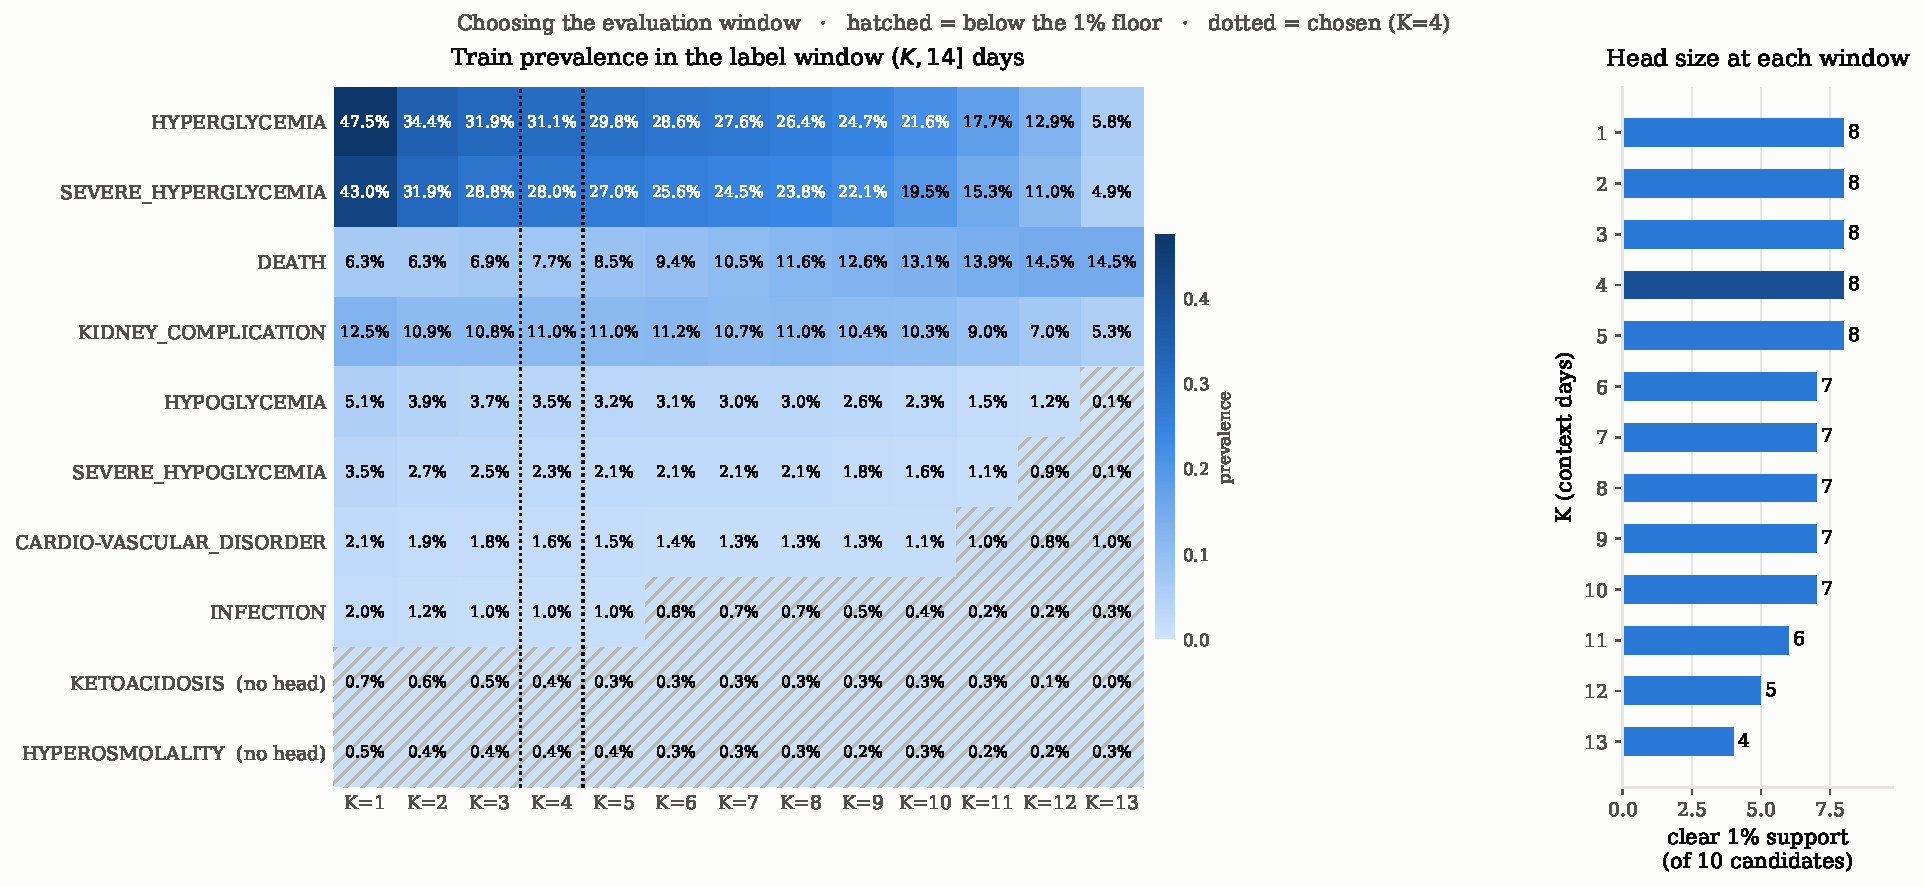
\includegraphics[width=\textwidth]{fig1_target_support}
\caption{Target support across candidate context windows on the Kineret
cohort. Prevalence is per admission on the training split; each candidate
target's line traces its prevalence as $K$ moves from $1$ to $13$ days.
The horizontal line at $1\%$ is the prevalence threshold; targets below
it at $K_{\mathrm{eval}}$ do not receive a prediction head.}
\label{fig:target-support}
\end{figure}

Figure~\ref{fig:target-support} shows the eight retained targets at
$K = 4$: hyperglycemia ($n_+ = 1{,}470$), severe hyperglycemia
($1{,}317$), kidney complication / AKI ($566$), $30$-day mortality
($341$), hypoglycemia ($181$), severe hypoglycemia ($111$), MI /
cardiovascular ($69$), and infection ($37$). Hyperosmolality
($n_+ \approx 220$, prevalence $\approx 0.44\%$) and ketoacidosis
($n_+ \approx 330$, $\approx 0.66\%$) fall below the $1\%$ threshold at
$K = 4$ and do not receive heads. Both would clear the threshold at
$K = 1$, but were excluded to hold the head layout fixed at the chosen
evaluation window; a target that flickers in and out of the head list
across arms would not admit a clean cross-arm comparison. Choosing the
window from this table before training keeps the results a single
support-conditioned table rather than a surface over $K$.

\subsection{The ladder}
\label{sec:results-ladder}

\begin{figure}[htbp]
\centering
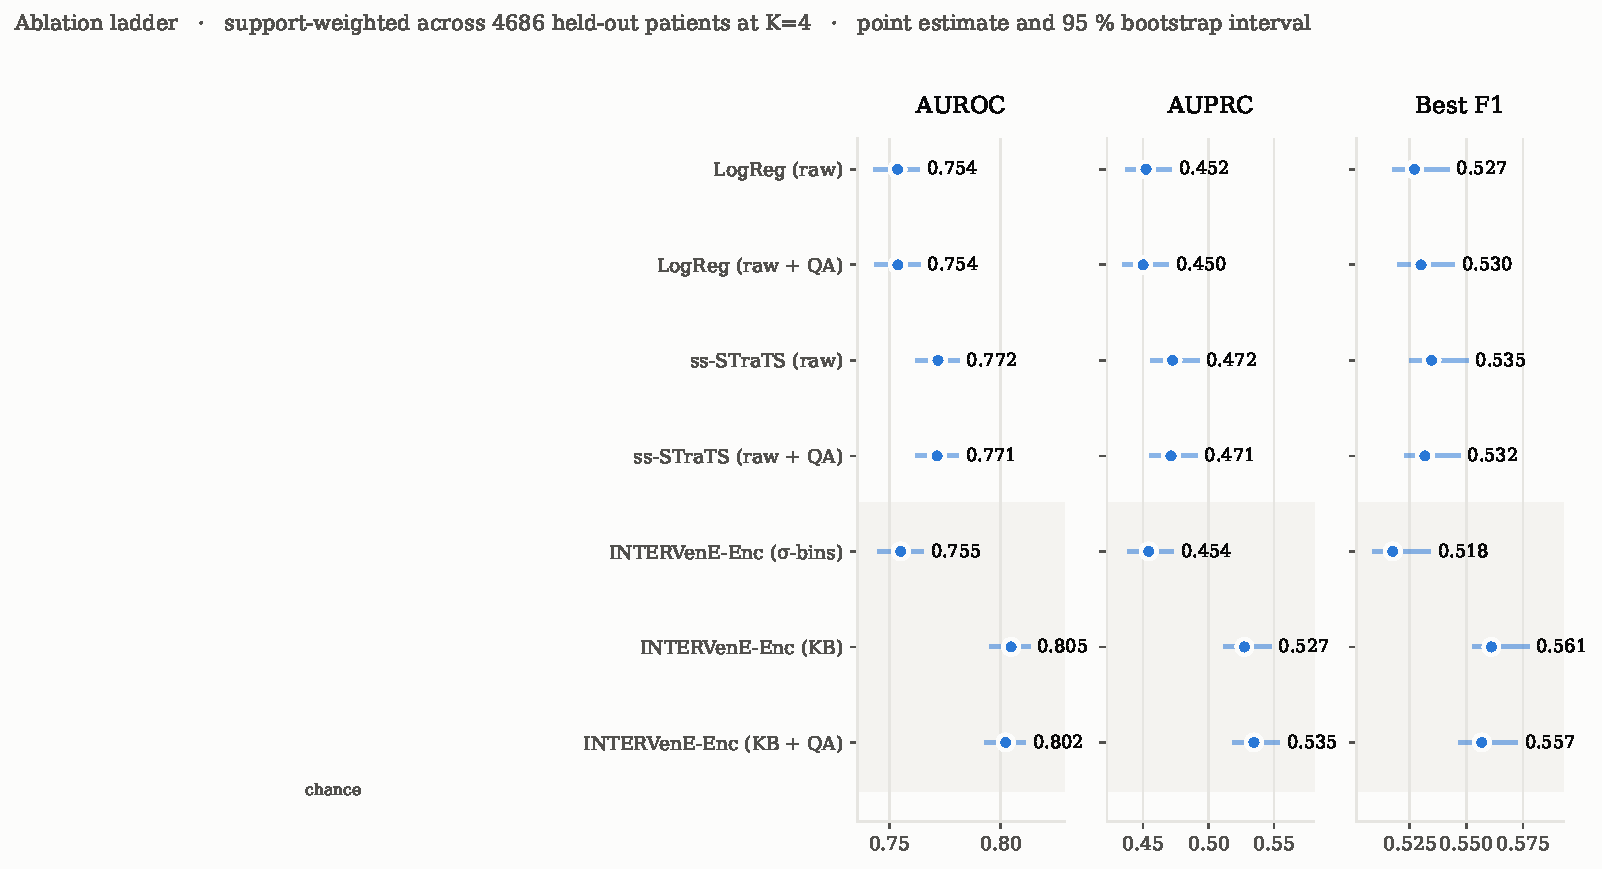
\includegraphics[width=\textwidth]{fig2_ladder}
\caption{Support-weighted performance across the seven arms on
$4{,}686$ held-out test admissions at $K = 4$, with $95\%$ patient-level
bootstrap intervals ($2{,}000$ resamples). Rungs $5\to 6$ isolate the
knowledge base; $6 \to 7$ the treatment-quality signal.}
\label{fig:ladder}
\end{figure}

\begin{table}[htbp]
\centering
\small
\caption{Support-weighted performance across the seven arms at $K = 4$.
Bold marks the best value in each column; brackets are $95\%$
patient-level bootstrap intervals.}
\label{tab:ladder}
\begin{tabular}{clccccc}
\toprule
Rung & Arm & AUROC & AUPRC & Best $F_1$ & Onset MAE (h) & LoS MAE (h) \\
\midrule
1 & LogReg                       & $0.754$ [$0.743,0.764$] & $0.452$ [$0.436,0.472$] & $0.527$          & $32.9$ & $47.7$ \\
2 & LogReg $+$ QA                & $0.754$ [$0.743,0.764$] & $0.450$ [$0.434,0.469$] & $0.530$          & $33.1$ & $47.7$ \\
3 & ss-STraTS                    & $0.772$ [$0.762,0.781$] & $0.472$ [$0.456,0.493$] & $0.535$          & $33.2$ & $46.4$ \\
4 & ss-STraTS $+$ QA             & $0.771$ [$0.762,0.781$] & $0.471$ [$0.455,0.491$] & $0.532$          & $32.8$ & $47.7$ \\
5 & INTERVenE-Enc ($\sigma$-bins)& $0.755$ [$0.744,0.765$] & $0.454$ [$0.438,0.473$] & $0.518$          & $33.3$ & $\mathbf{45.1}$ \\
6 & \textbf{INTERVenE-Enc (KB)}  & $\mathbf{0.805}$ [$0.795,0.813$] & $0.527$ [$0.511,0.548$] & $\mathbf{0.561}$ & $\mathbf{30.8}$ & $45.9$ \\
7 & INTERVenE-Enc (KB $+$ QA)    & $0.802$ [$0.793,0.811$] & $\mathbf{0.535}$ [$0.518,0.554$] & $0.557$ & $30.9$ & $46.0$ \\
\bottomrule
\end{tabular}
\end{table}

The architecture transfers. INTERVenE-Enc on knowledge-based
abstractions leads every arm on AUROC, best $F_1$ and onset error, at a
support-weighted AUPRC of $0.527$ against $0.472$ for the best
raw-stream baseline (ss-STraTS), with non-overlapping bootstrap
intervals (Table~\ref{tab:ladder}, Figure~\ref{fig:ladder}). The
KB $+$ QA arm edges KB alone on AUPRC ($0.535$ vs $0.527$), separated
by less than one interval width; the QA delta is decomposed in
Section~\ref{sec:results-qa}.

\paragraph{The knowledge base is doing predictive work.}
Replacing KBTA with $\sigma$-bin discretization (rung $5$) costs $0.073$
AUPRC and $0.050$ AUROC relative to rung $6$, and drops the arm to the
logistic-regression floor. The same substitution on MIMIC-IV
\citep{oded2027intervene} was within noise---the ablation there
attributed accuracy on that cohort to the Transformer over persistent
intervals rather than to the semantic content of the intervals. On the
data the knowledge base was authored for, that no longer holds:
clinical knowledge is doing predictive work, not only interpretive
work.

\paragraph{The architecture matters beyond having intervals.}
The floor is comfortably above chance ($0.754$ AUROC, $0.452$ AUPRC),
and ss-STraTS lifts AUROC and AUPRC only modestly over it ($+0.018$
AUROC, $+0.020$ AUPRC, both intervals overlapping the LogReg CI at the
lower end). The dominant modelling gain in the ladder is $6-3$: the
Transformer over KBTA intervals over the Transformer over triplets
($+0.033$ AUROC, $+0.055$ AUPRC, non-overlapping). Rungs $5-3$, which
compares the same INTERVenE-Enc architecture on $\sigma$-bins against
ss-STraTS on the raw stream, is within noise---the interval-based
Transformer is not intrinsically stronger, it becomes so once the
intervals carry named clinical concepts.

\paragraph{Length of stay.}
The $\sigma$-bin arm has the lowest length-of-stay error ($45.1$\,h),
below both KB arms ($45.9$--$46.0$\,h) and the raw-data arms
($46.4$--$47.7$\,h). Onset and length-of-stay heads share only the
encoder; the $\sigma$-bin encoder yields a marginally better LoS
signal despite the weakest risk performance. Onset is where the KB
arms separate cleanly: $30.8$\,h vs $32.9$--$33.3$\,h for every
raw-stream and $\sigma$-bin arm, a $\sim 2$\,h tightening that
survives bootstrap.

\subsection{The quality-assessment signal}
\label{sec:results-qa}

\begin{figure}[htbp]
\centering
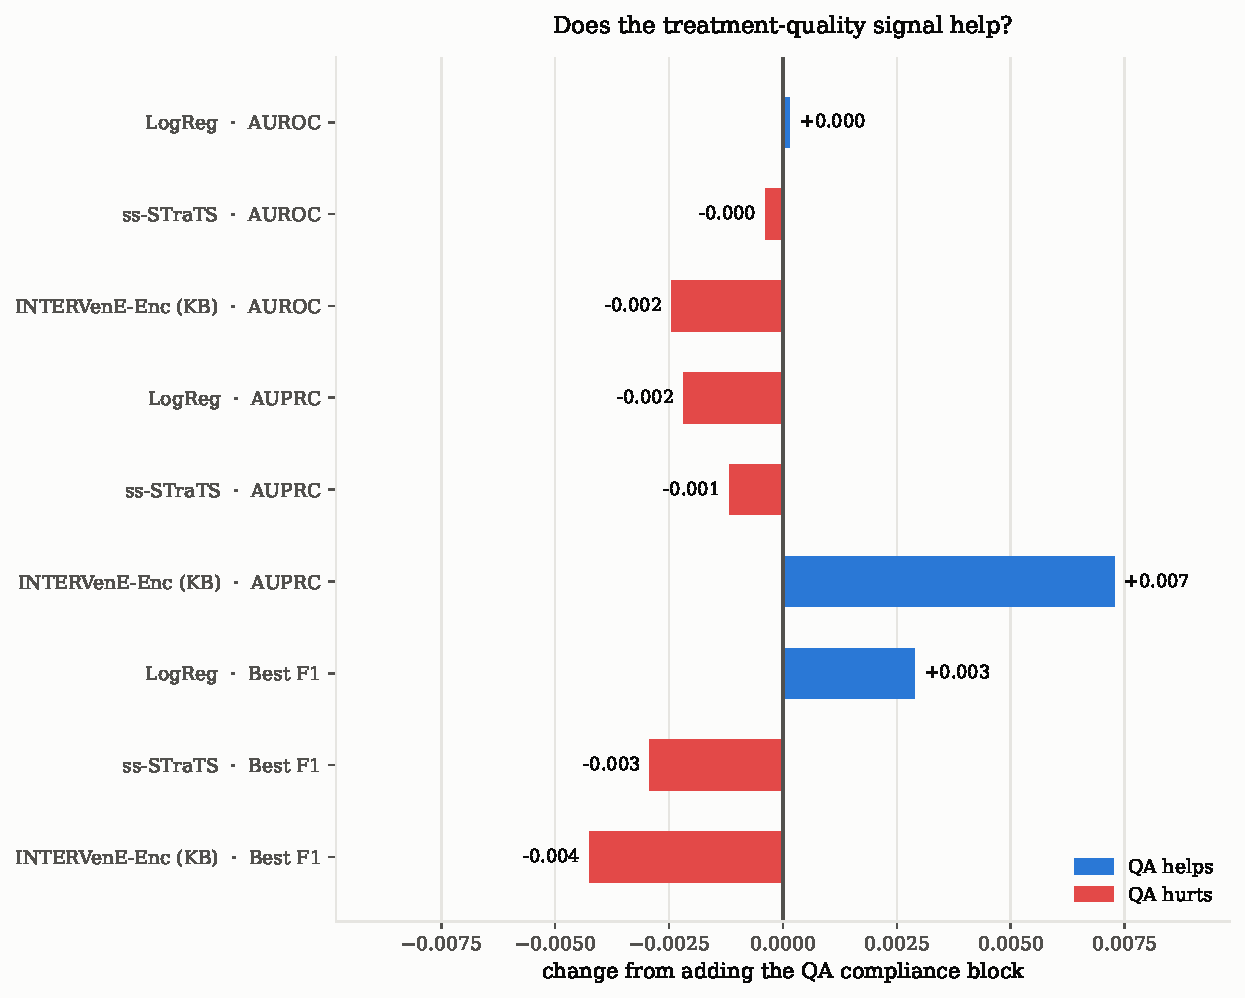
\includegraphics[width=0.85\textwidth]{fig3_qa_delta}
\caption{Change in support-weighted metrics from adding the aggregated
QA compliance block, per model. Positive values favour QA; error bars
are $95\%$ bootstrap intervals for the delta.}
\label{fig:qa-delta}
\end{figure}

Not measurably in aggregate. Every change sits at the third decimal
place with overlapping intervals (Figure~\ref{fig:qa-delta}). The
largest single change is INTERVenE-Enc's $+0.007$ AUPRC, and it is the
only arm that receives the compliance patterns as temporal tokens
rather than only as context.

The model \emph{does} use them. Sparse-transcoder attribution on the
QA arm, following the pipeline of \citep{oded2027intervene}, puts
\texttt{*\_PATTERN} tokens among the top drivers for seven of the
eight outcomes on this cohort: routine glucose monitoring for death
and kidney complication, basal-dosage and metformin-continuation
patterns for the glycemic endpoints, and reduced basal insulin after
hypoglycemia for severe hypoglycemia (attribution figure reproduced
from the concurrent methodological analysis; not shown here to
preserve the AIIM figure budget---see~\TODO{figure decision}). The
signal is read and assigned weight; it simply does not change the
aggregate metrics.

The interpretation is straightforward. The QA scores are derived
deterministically by the same abstraction engine that emits the
intervals the model is already reading; a model that reads
\emph{Glucose measured at $t$, insulin administered at $t + \delta$}
is close to computing \emph{compliance with insulin-following-
hyperglycemia at $t$} itself. The added signal is available and
used, but carries little the interval stream does not.

\subsection{Per-outcome results}
\label{sec:results-per-target}

\begin{figure}[htbp]
\centering
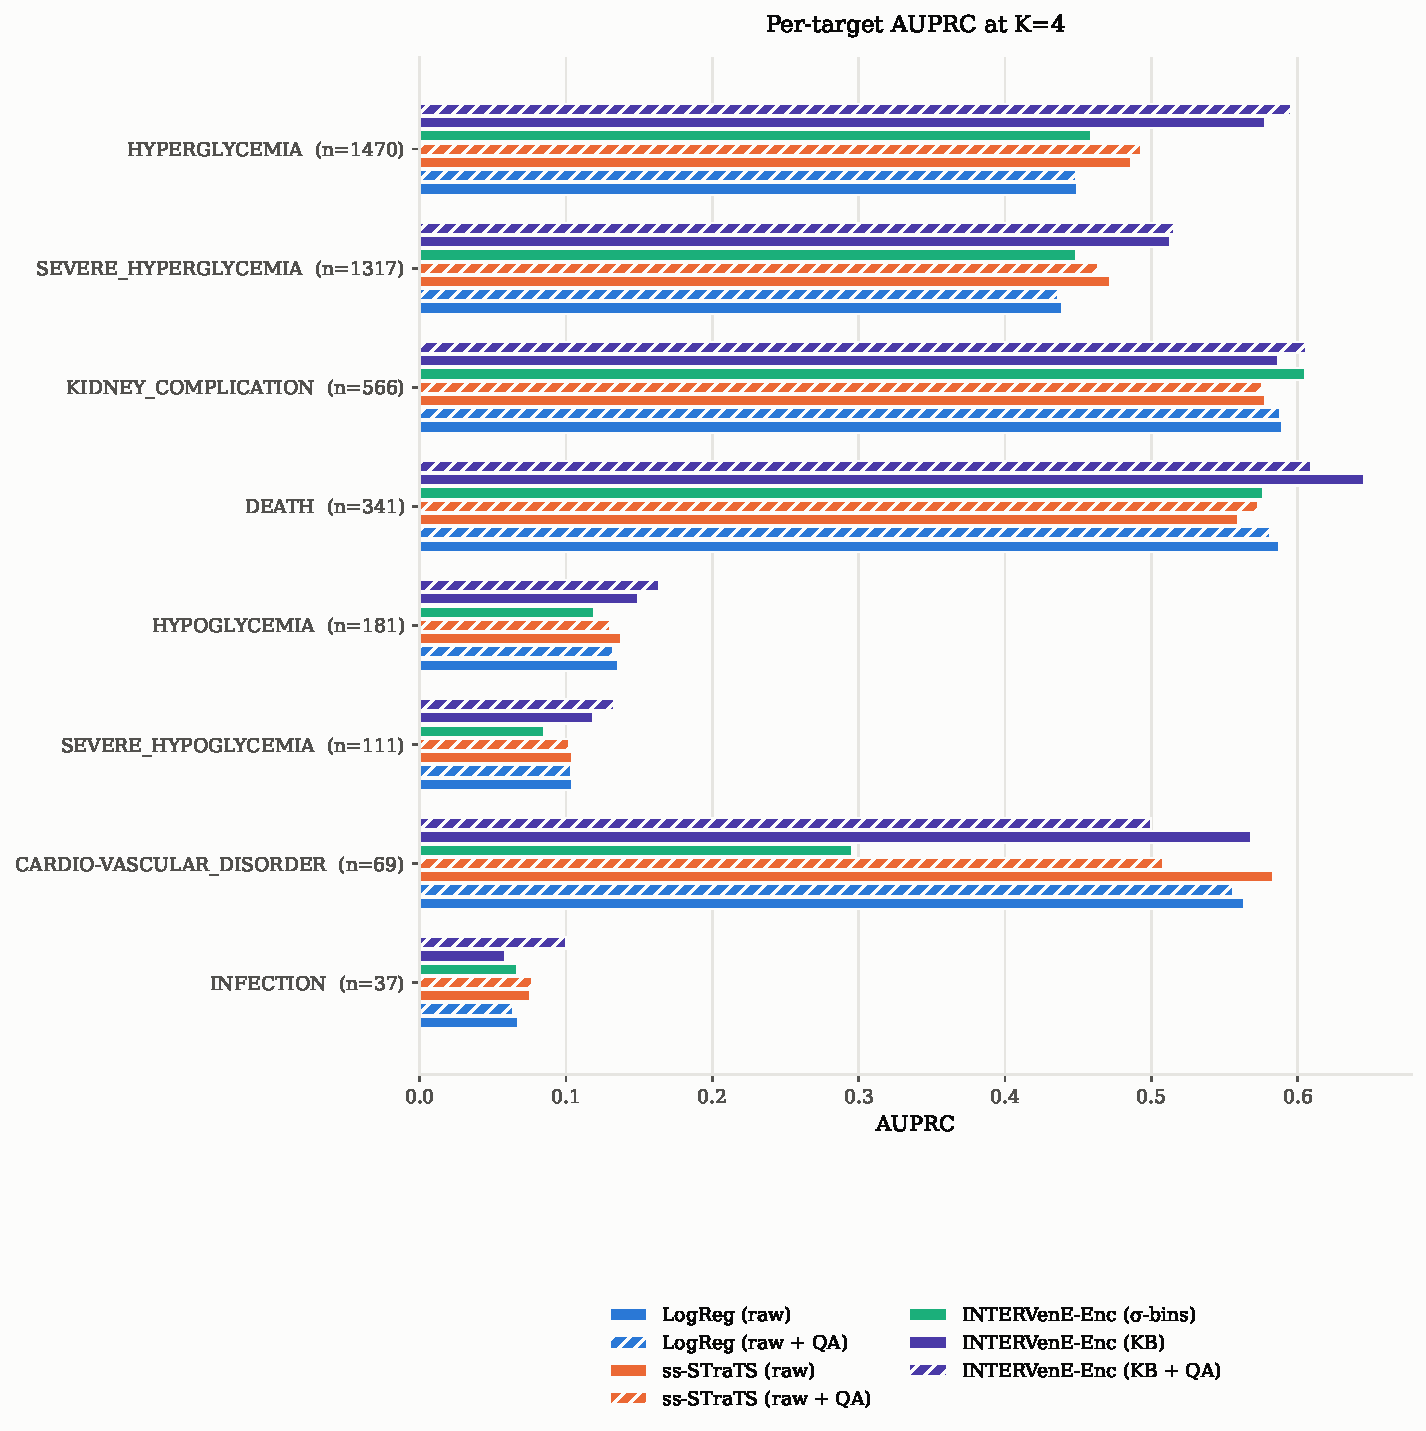
\includegraphics[width=\textwidth]{fig4_per_target_auprc}
\caption{Per-outcome AUPRC across the seven arms, ordered left-to-right
by positive count on the test set (dashed grey line: outcome
prevalence, the AUPRC random baseline).}
\label{fig:per-target-auprc}
\end{figure}

\begin{table}[htbp]
\centering
\small
\caption{Per-outcome AUPRC at $K = 4$, ordered by positive count. LR is
logistic regression, ST is ss-STraTS, $\sigma$ is INTERVenE-Enc on
$\sigma$-bins, KB and KB$+$QA the knowledge-based arms. Bold marks the
best value in each row; AKI is acute kidney injury; MI, myocardial
infarction.}
\label{tab:per-outcome}
\begin{tabular}{lrccccccc}
\toprule
Outcome & $n_+$ & LR & LR+QA & ST & ST+QA & $\sigma$ & KB & KB+QA \\
\midrule
Hyperglycemia         & 1{,}470 & 0.450 & 0.449 & 0.486 & 0.493 & 0.459 & 0.578 & \textbf{0.595} \\
Severe hyperglycemia  & 1{,}317 & 0.439 & 0.436 & 0.472 & 0.463 & 0.449 & 0.513 & \textbf{0.516} \\
AKI / kidney compl.   &   566   & 0.590 & 0.588 & 0.578 & 0.576 & 0.605 & 0.587 & \textbf{0.606} \\
Death                 &   341   & 0.587 & 0.581 & 0.559 & 0.573 & 0.577 & \textbf{0.645} & 0.609 \\
Hypoglycemia          &   181   & 0.135 & 0.132 & 0.138 & 0.130 & 0.119 & 0.149 & \textbf{0.163} \\
Severe hypoglycemia   &   111   & 0.104 & 0.103 & 0.104 & 0.102 & 0.085 & 0.119 & \textbf{0.133} \\
MI / cardiovascular   &    69   & 0.564 & 0.556 & \textbf{0.583} & 0.508 & 0.295 & 0.568 & 0.500 \\
Infection             &    37   & 0.067 & 0.064 & 0.076 & 0.077 & 0.067 & 0.058 & \textbf{0.100} \\
\bottomrule
\end{tabular}
\end{table}

The aggregate ordering is carried by the two frequent glycemic outcomes,
where the knowledge-based arms gain most: hyperglycemia $0.578$ against
$0.486$ for ss-STraTS, severe hyperglycemia $0.513$ against $0.472$.
Death is the only outcome where KB without QA leads outright ($0.645$).
Hyperglycemia is a lab-threshold event by definition; the KB collapses
$100$-plus glucose lab codes and $10$-plus insulin drugs into a single
\emph{glucose-state} and a single \emph{basal-insulin-context} channel,
and the model reads the abstraction directly. For death, no single
threshold defines the outcome, and the lift ($+0.086$ over ss-STraTS)
suggests the model is composing evidence across several
abstracted states.

Below roughly $200$ positives, the arms stop separating. Infection ($37$
positives), MI/cardiovascular ($69$) and severe hypoglycemia ($111$)
sit near their prevalence floors throughout, and the single largest
swing in the table---the $\sigma$-bin arm at $0.295$ on MI/cardiovascular
against $0.564$ for logistic regression---rests on $69$ events and
should not be read as an ordering. Weighting all eight outcomes equally
rather than by support lowers every figure (macro AUPRC $0.332$ to
$0.403$) but leaves the ranking of the arms unchanged.

\subsection{Onset and length of stay}

\begin{figure}[htbp]
\centering
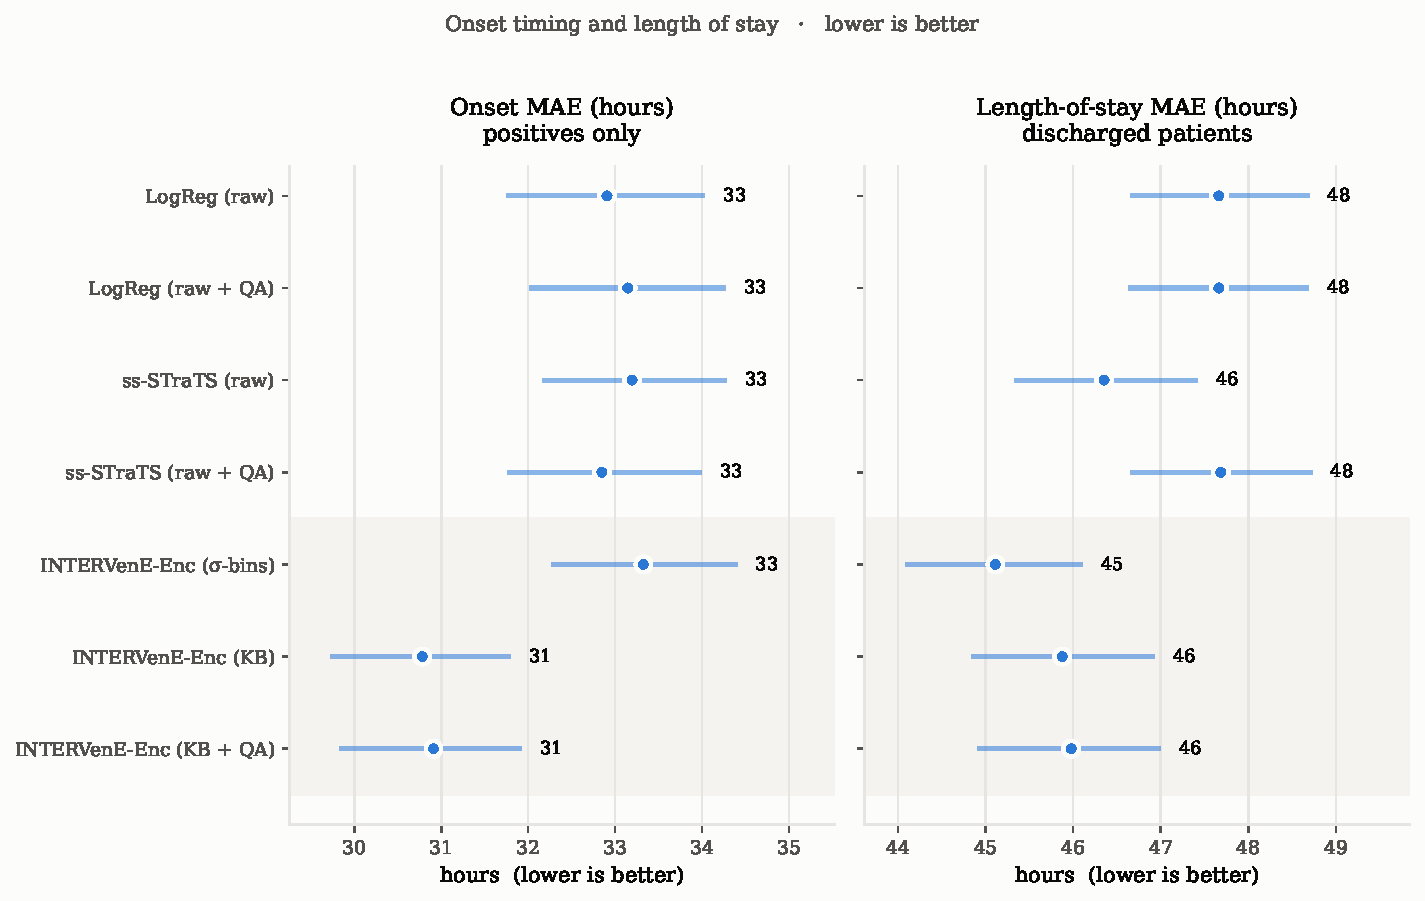
\includegraphics[width=\textwidth]{fig5_onset_and_los}
\caption{Onset MAE (hours, positives only) and length-of-stay MAE
(hours) per arm at $K = 4$. Onset is aggregated across outcomes by
support weighting; length of stay is a single regression head.
Error bars are $95\%$ bootstrap intervals.}
\label{fig:onset-los}
\end{figure}

Onset error tightens by $\sim 2$\,hours for the KB arms ($30.8$--$30.9$\,h)
relative to the raw-stream and $\sigma$-bin arms ($32.9$--$33.3$\,h;
Figure~\ref{fig:onset-los}). Length of stay error is close across the
ladder ($45.1$--$47.7$\,h), and does not track risk performance: the
$\sigma$-bin arm has the lowest LoS despite the weakest risk metrics,
because the two heads share only the encoder. The KB arms $6$ and $7$
sit essentially on top of one another for both time heads, consistent
with QA leaving aggregate metrics untouched.

\section{Discussion}
\label{sec:discussion}

\subsection{Principal findings}

\paragraph{The architecture transfers.}
INTERVenE-Enc, tuned and evaluated on MIMIC-IV ICU-level data
\citep{oded2027intervene}, retains its ordering against strong raw-stream
baselines on a very different cohort: multicenter, general ward, older,
longer stays, and shorter observation window in relative terms (K = 4 of
14 days here versus K = 2 of 14 days on MIMIC). No hyperparameters were
tuned to this cohort. Support-weighted AUPRC lifts from $0.472$ for
ss-STraTS to $0.527$ for INTERVenE-Enc on KBTA, with non-overlapping
bootstrap intervals---a similar relative gap to the MIMIC-IV finding
($0.631 \to 0.672$).

\paragraph{The knowledge base does more here than on MIMIC-IV.}
The single most informative contrast in the paper is the $\sigma$-bin
arm against the KB arm ($5 \to 6$): identical Transformer, identical
data, identical labels, replacing only the abstraction layer with a
seven-band $\sigma$-discretization. On MIMIC-IV that substitution was
within noise \citep{oded2027intervene}; on Kineret it costs $0.073$
AUPRC ($0.454 \to 0.527$) and $0.050$ AUROC, and drops the arm to the
logistic-regression floor. The interpretation is that a knowledge base
authored for the diabetes-inpatient network it is deployed on carries
predictive information that a knowledge-free discretization does not
recover---even when the discretization is fed to the same
Transformer.

Two related observations follow. First, this is where clinical domain
knowledge and empirical modelling meet materially: the same authors
constructed the abstraction rules \citep{hochberg2023inpatient} that
give this arm its lift and are unavailable to $\sigma$-bins. Second,
knowledge-base contribution to accuracy is cohort-dependent, and
studies of the value of clinical knowledge in EHR modelling that
report a single dataset (MIMIC or otherwise) should be read
accordingly.

\paragraph{Measured guideline adherence does not shift aggregate
metrics.}
The QA contribution is bounded by $\le 0.008$ on any aggregate metric
across three architectures (Figure~\ref{fig:qa-delta}). The signal is
used---sparse-transcoder attribution places compliance-pattern tokens
among the top drivers for seven of eight outcomes---but is largely
redundant with the interval stream a KB-consuming model is already
reading, because both are deterministic derivations of the same
underlying abstraction engine. The concurrent adherence study
\citep{oded2027kineret-jbi} identified above-median adherence as
associated with lower mortality (OR $=0.557$ after propensity
weighting); those population-level associations do not need to
translate to per-admission predictive lift for a model already reading
the underlying abstractions.

This has a design consequence. If a downstream task cares about the
score \emph{as an operational input}---e.g., a dashboard alerting on
low compliance---the QA layer stands on its own on its aggregation
target. If the task is complication prediction from a model that
already consumes the abstractions, no additional AUPRC accrues from
supplying the score. Which of the two the deployment cares about
determines whether the QA layer is a predictor input, a monitoring
readout, or both.

\subsection{The design that let both questions be answered}

Two decisions distinguish this study from an ordinary architecture
comparison.

\paragraph{One canonical event set.}
Complications appear in two source tables: the raw table
(\texttt{mediator\_input.csv}, containing the measurements the
knowledge base reads) and the Mediator output (containing its verdicts).
These disagree on which occurrences happened and when, both because
measurement-derived rules were not authored twice and because timestamps
drift by minutes across derivations. We rebuild the raw side's own
complication rows in Python by applying the same threshold rules the
Mediator's XML applies, then intersect the two views at $1$-minute
tolerance and keep only occurrences the two files date identically. The
result is one canonical event set that supplies labels, is re-injected
into every arm's input stream, and is asserted by a unit test to be
identical across arms. Without this step, on this cohort, the raw file
carried zero lab-threshold complications and the Mediator carried
$68{,}525$; cross-file alignment of the pre-computed complications
found a support drift of $3{,}096$ vs $3{,}098$ / $2{,}849$ vs $2{,}854$
that would otherwise have made \emph{which events did each arm see} a
confound rather than a constant.

\paragraph{Knowledge containment.}
The Mediator emits \texttt{*\_EVENT} concepts that are not prediction
targets---\texttt{AKI\_EVENT}, \texttt{ELECTROLYTE\_DERANGEMENT\_EVENT},
\texttt{MYOCARDIAL\_INJURY\_EVENT}. Each is a knowledge-base verdict
reached by reading raw measurements. Handing them to LogReg or
ss-STraTS would give those arms clinical judgements they could not have
computed themselves, and rungs $5 \to 6$ would then measure a leak
rather than the abstraction lift. The two streams differ by design:
non-target \texttt{*\_EVENT} concepts are stripped from the raw stream
and kept in the KB stream; target events go to everyone as observed
history. This is the one place a wiring mistake would silently
invalidate every cross-arm number in the paper, so it is asserted by a
unit test in both directions.

\subsection{Where the knowledge base helps most}

The KB arm's largest per-outcome lifts are on the two frequent glycemic
outcomes---hyperglycemia $0.578$ over ss-STraTS $0.486$ ($+0.092$
AUPRC); severe hyperglycemia $0.513$ over $0.472$ ($+0.041$). These are
threshold events by definition: hyperglycemia is a glucose level above
a defined cut, and the knowledge base collapses hundreds of lab codes
into a single \emph{glucose-state} channel with the threshold applied.
The model reads the clinical definition of its label directly, which is
close to what an interpretable clinical scoring rule would do.

Death is more interesting: no single KBTA threshold defines it, and the
lift ($0.645$ vs $0.559$ for ss-STraTS) suggests the model composes
evidence across several abstracted states. This is consistent with the
sparse-transcoder attribution reported on MIMIC-IV, which found
hypoalbuminemia (a chronic-mortality marker), aminotransferase
elevation (liver stress), and bicarbonate shifts (acid--base
decompensation) as the top death drivers. The same clinical logic---
composition across abstracted trends rather than reading a single
threshold---applies to LoS ($44.4$\,h vs $\sim 48$\,h on MIMIC-IV,
$45.9$\,h vs $46.4$\,h here).

Below roughly $200$ positives, the arms stop separating: infection,
MI/cardiovascular, and severe hypoglycemia sit near their prevalence
floors regardless of arm, and the single largest swing in the per-
outcome table---the $\sigma$-bin arm at $0.295$ on MI/cardiovascular
against $0.564$ for logistic regression---rests on $69$ events and
should not be read as an ordering. This is a study-power finding rather
than a modelling one: the cohort under-samples rare complications in
absolute terms, and running a larger extract would sharpen those rows
without needing any change to the pipeline.

\subsection{Limitations}
\label{sec:discussion-limits}

\paragraph{One cohort, single-seed training.}
Every arm is trained once, at the reference-repository hyperparameters,
without a per-cohort tune. Multi-seed variance was not affordable
inside the regulated environment; the reported bootstrap intervals
capture sampling variability for the fitted model, not the variance of
the training procedure. This is the same limitation reported by the
methodological MIMIC-IV study \citep{oded2027intervene}.

\paragraph{External validity is limited.}
This is the second cohort INTERVenE has been evaluated on, and both are
diabetic. Whether the architecture-transferred and knowledge-lift-larger
findings extend to non-diabetic complication prediction, or to
non-Israeli hospital networks, is not settled here---though the design
of the ladder is portable and the release of the code
(Section~\ref{sec:reproducibility}) makes the experiment repeatable
elsewhere.

\paragraph{The knowledge base itself is not evaluated here.}
The knowledge base used to produce the KB stream is the diabetes-
inpatient ontology of \citep{hochberg2023inpatient,oded2027kineret-jbi};
this paper takes it as given. Its predictive contribution is what rungs
$5 \to 6$ measure, but the ontology's coverage, calibration and edge
cases are the subject of the concurrent adherence study, not this one.

\paragraph{Class imbalance at the tail of the target list.}
Four of the eight targets have fewer than $200$ positives on the test
set. Their intervals overlap across most arms and their per-outcome
comparisons should not be over-read. This is not a modelling artefact
but a data-scale one; a larger extract would resolve it.

\paragraph{Model calibration is not reported.}
Reliability curves and expected calibration error were computed on the
MIMIC-IV cohort and reported per outcome in
\citep{oded2027intervene}. We omit the corresponding analysis here to
stay inside the AIIM figure budget, but the run-outputs contain the
per-prediction probabilities needed to reproduce them
(Section~\ref{sec:reproducibility}); this is~\TODO{a candidate for the
supplementary material.}

\paragraph{No temporal or per-hospital held-out.}
The split is patient-level and random. The concurrent adherence study
demonstrated a small but measurable shift in adherence patterns after
the 2023 guideline was issued, and a temporal-holdout evaluation
(train pre-guideline, test post-guideline, or vice versa) would test
whether prediction quality tracks that shift. Similarly, a per-hospital
leave-one-out would test whether the model generalizes across sites
within the network. Both are~\TODO{listed as open reviewer questions in
Section~\ref{sec:tasks-open} of the draft appendix.}

\section{Conclusion}
\label{sec:conclusion}

A seven-arm ladder that varies only the input representation---holding
cohort, labels, patient split, evaluation window and head layout
constant---separates the effect of the neural architecture, the effect
of the clinical knowledge base, and the effect of a
guideline-adherence signal, on a multicenter inpatient-diabetes cohort.

Three findings follow. The interval-based Transformer INTERVenE-Enc
transfers to a second cohort without hyperparameter retuning, keeping
its ordering over ss-STraTS and logistic-regression baselines with
non-overlapping bootstrap intervals. The knowledge base contributes
$0.073$ AUPRC over a knowledge-free $\sigma$-bin discretization---an
effect that was within noise on MIMIC-IV---so clinical domain knowledge
does predictive work on data it was authored for, not merely
interpretive work. Automatically measured guideline adherence, computed
by the same abstraction engine that produces the intervals the model
already reads, is used by the model but does not shift aggregate
metrics; QA is close to what a KB-consuming model extracts for itself.

The design that let these three effects be measured cleanly is
transferable, and the release of the code, the frozen configuration and
the per-arm predictions makes the same experiment repeatable on a
different network with a different knowledge base. Whether the
architecture-transferred and knowledge-lift-larger findings extend to
non-diabetic prediction, and whether adherence signals help
prediction where a knowledge base is \emph{not} in the model's input,
are the two questions this ladder leaves for follow-on work.

\section*{Reproducibility}
\label{sec:reproducibility}

Every number and every figure in this paper is produced by running
\texttt{notebooks/benchmark.ipynb} in the Kineret-Prediction repository
against the frozen \texttt{study\_config.json} shipped with it. The
per-arm predictions, per-outcome metrics, bootstrap intervals and
figures are additionally shipped as \texttt{results/full\_bench\_results/}
in the same repository. The abstraction engine, the ETL pipeline, and
both reference implementations (INTERVenE-Enc, ss-STraTS) are separately
released; see the \emph{Data and Code Availability} statement.


\section*{CRediT Authorship Contribution Statement}
\textbf{Shahar Oded:} Conceptualization, Methodology, Software, Validation,
Formal analysis, Data curation, Visualization, Writing---original draft.
\textbf{Yuval Shahar:} Conceptualization, Methodology, Supervision, Funding
acquisition, Writing---review \& editing.
\textbf{Erez Shalom:} Resources, Project administration, Writing---review \&
editing.
\textbf{Amir Bashkin:} Investigation, Resources, Writing---review \& editing.
\textbf{Leonard Saig:} Investigation, Resources, Writing---review \& editing.
\textbf{Dror Cantrell:} Investigation, Resources, Writing---review \& editing.
\textbf{Irit Wirsansky:} Investigation, Resources, Writing---review \& editing.
\textbf{Muhamad Badarne:} Investigation, Resources, Writing---review \& editing.
\textbf{Irena Barash:} Investigation, Resources, Writing---review \& editing.
\textbf{Avivit Cahn:} Conceptualization, Investigation, Writing---review \&
editing.
\textbf{Irit Hochberg:} Conceptualization, Methodology, Validation,
Resources, Supervision, Writing---review \& editing.

\section*{Funding}
\TODO{Funding statement outstanding --- to be aligned with the JBI/JAMIA
companion papers.}

\section*{Declaration of Competing Interest}
Several of the authors contributed to the national position paper whose
implementation informs the QA arm of this study. The authors declare no
competing financial interests or personal relationships that could have
appeared to influence the work reported in this paper.

\section*{Data and Code Availability}
The Mediator abstraction engine and its knowledge base, the extraction and
cohort-construction pipeline, the seven-arm benchmark, and the frozen
outputs used to produce every table and figure in this paper are publicly
available:

\begin{itemize}\setlength{\itemsep}{.1em}
\item Mediator (abstraction + quality-assessment engine):
      \url{https://github.com/shaharoded/Mediator}.
\item Kineret ETL pipeline (OMOP CDM $\to$ analysis-ready tables):
      \url{https://github.com/shaharoded/Kineret-ETL}.
\item INTERVenE-Enc reference implementation:
      \url{https://github.com/shaharoded/INTERVenE-Enc}.
\item ss-STraTS reference implementation:
      \url{https://github.com/shaharoded/Medical-Transformers-Benchmark}.
\item This study's pipeline, frozen configuration, per-arm predictions,
      per-outcome bootstraps and figures:
      \url{https://github.com/shaharoded/Kineret-Prediction} (see
      \texttt{results/full\_bench\_results/}).
\end{itemize}

All processing was performed inside a closed hospital computing environment.
The code released is a replica of that pipeline; no source data,
intermediate datasets, or unaggregated outputs leave that environment.
Reported results are exported aggregate statistics. The patient-level EHR
data cannot be shared, as it comprises identifiable clinical records
governed by the approvals under which it was obtained.

\section*{Ethics Approval}
The study was approved by the institutional Helsinki committee of each
participating center under a common protocol (NHR-0152-23): Galilee Medical
Center (NHR-0152-23), Hillel Yaffe Medical Center (HYMC-0074-24), Shamir
Medical Center (ASF-0117-24), Tzafon Medical Center (POR-0047-24), Barzilai
University Medical Center (BRZ-0059-24), and Bnai Zion Medical Center
(BNZ-0067-24). A full waiver of informed consent was granted, since the
study extracts records from a de-identified repository with no patient
contact.

\section*{Acknowledgements}
This study rests on the Kineret project team, who built and maintain the
harmonized multicenter data warehouse. The authors also thank the Helsinki
committee coordinators at the participating centers for their assistance
throughout the approval process.

\bibliographystyle{elsarticle-num}
\bibliography{references}

\end{document}
